% Options for packages loaded elsewhere
\PassOptionsToPackage{unicode}{hyperref}
\PassOptionsToPackage{hyphens}{url}
\PassOptionsToPackage{dvipsnames,svgnames,x11names}{xcolor}
%
\documentclass[
  letterpaper,
  DIV=11,
  numbers=noendperiod]{scrartcl}

\usepackage{amsmath,amssymb}
\usepackage{iftex}
\ifPDFTeX
  \usepackage[T1]{fontenc}
  \usepackage[utf8]{inputenc}
  \usepackage{textcomp} % provide euro and other symbols
\else % if luatex or xetex
  \usepackage{unicode-math}
  \defaultfontfeatures{Scale=MatchLowercase}
  \defaultfontfeatures[\rmfamily]{Ligatures=TeX,Scale=1}
\fi
\usepackage{lmodern}
\ifPDFTeX\else  
    % xetex/luatex font selection
\fi
% Use upquote if available, for straight quotes in verbatim environments
\IfFileExists{upquote.sty}{\usepackage{upquote}}{}
\IfFileExists{microtype.sty}{% use microtype if available
  \usepackage[]{microtype}
  \UseMicrotypeSet[protrusion]{basicmath} % disable protrusion for tt fonts
}{}
\makeatletter
\@ifundefined{KOMAClassName}{% if non-KOMA class
  \IfFileExists{parskip.sty}{%
    \usepackage{parskip}
  }{% else
    \setlength{\parindent}{0pt}
    \setlength{\parskip}{6pt plus 2pt minus 1pt}}
}{% if KOMA class
  \KOMAoptions{parskip=half}}
\makeatother
\usepackage{xcolor}
\setlength{\emergencystretch}{3em} % prevent overfull lines
\setcounter{secnumdepth}{-\maxdimen} % remove section numbering
% Make \paragraph and \subparagraph free-standing
\ifx\paragraph\undefined\else
  \let\oldparagraph\paragraph
  \renewcommand{\paragraph}[1]{\oldparagraph{#1}\mbox{}}
\fi
\ifx\subparagraph\undefined\else
  \let\oldsubparagraph\subparagraph
  \renewcommand{\subparagraph}[1]{\oldsubparagraph{#1}\mbox{}}
\fi

\usepackage{color}
\usepackage{fancyvrb}
\newcommand{\VerbBar}{|}
\newcommand{\VERB}{\Verb[commandchars=\\\{\}]}
\DefineVerbatimEnvironment{Highlighting}{Verbatim}{commandchars=\\\{\}}
% Add ',fontsize=\small' for more characters per line
\usepackage{framed}
\definecolor{shadecolor}{RGB}{241,243,245}
\newenvironment{Shaded}{\begin{snugshade}}{\end{snugshade}}
\newcommand{\AlertTok}[1]{\textcolor[rgb]{0.68,0.00,0.00}{#1}}
\newcommand{\AnnotationTok}[1]{\textcolor[rgb]{0.37,0.37,0.37}{#1}}
\newcommand{\AttributeTok}[1]{\textcolor[rgb]{0.40,0.45,0.13}{#1}}
\newcommand{\BaseNTok}[1]{\textcolor[rgb]{0.68,0.00,0.00}{#1}}
\newcommand{\BuiltInTok}[1]{\textcolor[rgb]{0.00,0.23,0.31}{#1}}
\newcommand{\CharTok}[1]{\textcolor[rgb]{0.13,0.47,0.30}{#1}}
\newcommand{\CommentTok}[1]{\textcolor[rgb]{0.37,0.37,0.37}{#1}}
\newcommand{\CommentVarTok}[1]{\textcolor[rgb]{0.37,0.37,0.37}{\textit{#1}}}
\newcommand{\ConstantTok}[1]{\textcolor[rgb]{0.56,0.35,0.01}{#1}}
\newcommand{\ControlFlowTok}[1]{\textcolor[rgb]{0.00,0.23,0.31}{#1}}
\newcommand{\DataTypeTok}[1]{\textcolor[rgb]{0.68,0.00,0.00}{#1}}
\newcommand{\DecValTok}[1]{\textcolor[rgb]{0.68,0.00,0.00}{#1}}
\newcommand{\DocumentationTok}[1]{\textcolor[rgb]{0.37,0.37,0.37}{\textit{#1}}}
\newcommand{\ErrorTok}[1]{\textcolor[rgb]{0.68,0.00,0.00}{#1}}
\newcommand{\ExtensionTok}[1]{\textcolor[rgb]{0.00,0.23,0.31}{#1}}
\newcommand{\FloatTok}[1]{\textcolor[rgb]{0.68,0.00,0.00}{#1}}
\newcommand{\FunctionTok}[1]{\textcolor[rgb]{0.28,0.35,0.67}{#1}}
\newcommand{\ImportTok}[1]{\textcolor[rgb]{0.00,0.46,0.62}{#1}}
\newcommand{\InformationTok}[1]{\textcolor[rgb]{0.37,0.37,0.37}{#1}}
\newcommand{\KeywordTok}[1]{\textcolor[rgb]{0.00,0.23,0.31}{#1}}
\newcommand{\NormalTok}[1]{\textcolor[rgb]{0.00,0.23,0.31}{#1}}
\newcommand{\OperatorTok}[1]{\textcolor[rgb]{0.37,0.37,0.37}{#1}}
\newcommand{\OtherTok}[1]{\textcolor[rgb]{0.00,0.23,0.31}{#1}}
\newcommand{\PreprocessorTok}[1]{\textcolor[rgb]{0.68,0.00,0.00}{#1}}
\newcommand{\RegionMarkerTok}[1]{\textcolor[rgb]{0.00,0.23,0.31}{#1}}
\newcommand{\SpecialCharTok}[1]{\textcolor[rgb]{0.37,0.37,0.37}{#1}}
\newcommand{\SpecialStringTok}[1]{\textcolor[rgb]{0.13,0.47,0.30}{#1}}
\newcommand{\StringTok}[1]{\textcolor[rgb]{0.13,0.47,0.30}{#1}}
\newcommand{\VariableTok}[1]{\textcolor[rgb]{0.07,0.07,0.07}{#1}}
\newcommand{\VerbatimStringTok}[1]{\textcolor[rgb]{0.13,0.47,0.30}{#1}}
\newcommand{\WarningTok}[1]{\textcolor[rgb]{0.37,0.37,0.37}{\textit{#1}}}

\providecommand{\tightlist}{%
  \setlength{\itemsep}{0pt}\setlength{\parskip}{0pt}}\usepackage{longtable,booktabs,array}
\usepackage{calc} % for calculating minipage widths
% Correct order of tables after \paragraph or \subparagraph
\usepackage{etoolbox}
\makeatletter
\patchcmd\longtable{\par}{\if@noskipsec\mbox{}\fi\par}{}{}
\makeatother
% Allow footnotes in longtable head/foot
\IfFileExists{footnotehyper.sty}{\usepackage{footnotehyper}}{\usepackage{footnote}}
\makesavenoteenv{longtable}
\usepackage{graphicx}
\makeatletter
\def\maxwidth{\ifdim\Gin@nat@width>\linewidth\linewidth\else\Gin@nat@width\fi}
\def\maxheight{\ifdim\Gin@nat@height>\textheight\textheight\else\Gin@nat@height\fi}
\makeatother
% Scale images if necessary, so that they will not overflow the page
% margins by default, and it is still possible to overwrite the defaults
% using explicit options in \includegraphics[width, height, ...]{}
\setkeys{Gin}{width=\maxwidth,height=\maxheight,keepaspectratio}
% Set default figure placement to htbp
\makeatletter
\def\fps@figure{htbp}
\makeatother

\usepackage{booktabs}
\usepackage{longtable}
\usepackage{array}
\usepackage{multirow}
\usepackage{wrapfig}
\usepackage{float}
\usepackage{colortbl}
\usepackage{pdflscape}
\usepackage{tabu}
\usepackage{threeparttable}
\usepackage{threeparttablex}
\usepackage[normalem]{ulem}
\usepackage{makecell}
\usepackage{xcolor}
\KOMAoption{captions}{tableheading}
\usepackage{geometry}
\geometry{left=1cm, right=1cm, top=1cm, bottom=1cm}
\usepackage{anyfontsize}
\fontsize{12}{15}\selectfont
\makeatletter
\@ifpackageloaded{caption}{}{\usepackage{caption}}
\AtBeginDocument{%
\ifdefined\contentsname
  \renewcommand*\contentsname{Table of contents}
\else
  \newcommand\contentsname{Table of contents}
\fi
\ifdefined\listfigurename
  \renewcommand*\listfigurename{List of Figures}
\else
  \newcommand\listfigurename{List of Figures}
\fi
\ifdefined\listtablename
  \renewcommand*\listtablename{List of Tables}
\else
  \newcommand\listtablename{List of Tables}
\fi
\ifdefined\figurename
  \renewcommand*\figurename{Figure}
\else
  \newcommand\figurename{Figure}
\fi
\ifdefined\tablename
  \renewcommand*\tablename{Table}
\else
  \newcommand\tablename{Table}
\fi
}
\@ifpackageloaded{float}{}{\usepackage{float}}
\floatstyle{ruled}
\@ifundefined{c@chapter}{\newfloat{codelisting}{h}{lop}}{\newfloat{codelisting}{h}{lop}[chapter]}
\floatname{codelisting}{Listing}
\newcommand*\listoflistings{\listof{codelisting}{List of Listings}}
\makeatother
\makeatletter
\makeatother
\makeatletter
\@ifpackageloaded{caption}{}{\usepackage{caption}}
\@ifpackageloaded{subcaption}{}{\usepackage{subcaption}}
\makeatother
\ifLuaTeX
  \usepackage{selnolig}  % disable illegal ligatures
\fi
\usepackage{bookmark}

\IfFileExists{xurl.sty}{\usepackage{xurl}}{} % add URL line breaks if available
\urlstyle{same} % disable monospaced font for URLs
\hypersetup{
  pdftitle={Final\_Project\_Paper},
  pdfauthor={Ben Lawrence},
  colorlinks=true,
  linkcolor={blue},
  filecolor={Maroon},
  citecolor={Blue},
  urlcolor={Blue},
  pdfcreator={LaTeX via pandoc}}

\title{Final\_Project\_Paper}
\author{Ben Lawrence}
\date{}

\begin{document}
\maketitle

\subsection{Data Description}\label{data-description}

We obtained the two datasets from the UC Irvine Machine Learning
Repository (UCIMLR). They were donated by authors, Paulo Cortez and
Alice Silva, of the article ``Using Data Mining to Predict Secondary
School Student Performance''. The authors belong to the University of
Minho in Portugal and were interested in model efficacy in the
prediction of the academic performance of Portuguese secondary
students.~

Each dataset aligns with a single subject, Portuguese and Mathematics,
collected from two Portuguese secondary schools. The Mathematics dataset
contains 395 observations and the Portuguese contains 649. They both
have 33 columns.~~

\hfill\break
Three of the columns are trimester grades of students with the third
trimester grade \textbf{G3} taken as the student's final grade. We will
take this as our response and the previous two trimester grades as
predictors. The remaining predictors consist of demographic survey data
acquired for each student observation. These include number of absences,
number of previous class failures, occupation of mother/father, etc.
Most of the variables are categorical, taking ordinal and nominative
values. There are also variables that take on binary and integer values.
We will begin our analysis by visualizing the distribution of
\textbf{G3} for the Mathematics and Portuguese data set.~

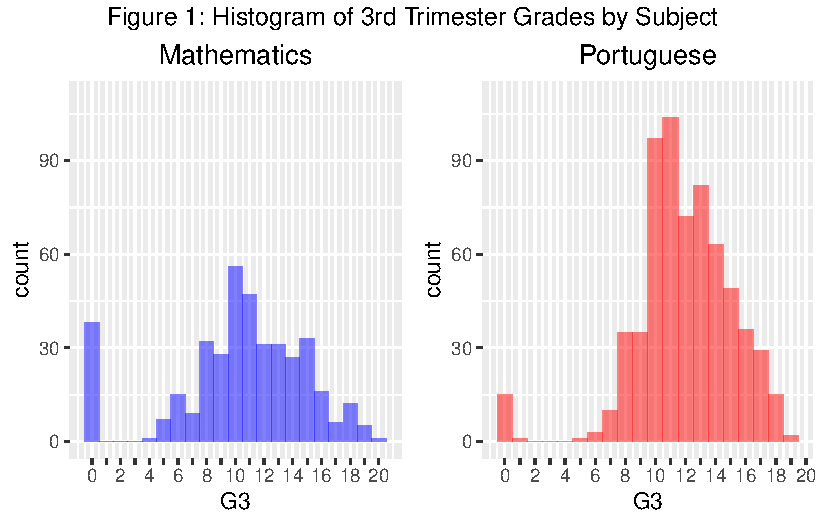
\includegraphics{Final_Paper_edit_files/figure-pdf/unnamed-chunk-1-1.pdf}

In Figure 1 we can observe that the grades are skewed to the right. This
is reasonable since we would expect a higher proportion of students
passing (scoring over 10) than failing. There is a notable set of
outlying points where a much higher proportion of students received 0s
than we would reasonably expect. This is especially true in the
mathematics class.

Figure 2 below provides examples of the predictors available in our
dataset. (Full list available HERE) We will use all of these in our full
linear model. Before creating such a model however, we will take time to
analyze the relationship between G1, G2, absences, and failures with the
response G3 to see if transformations of these variables are warranted.
The other variables are categorical and do not offer obvious visual
correlations with G3 that can inform our transformation choices.

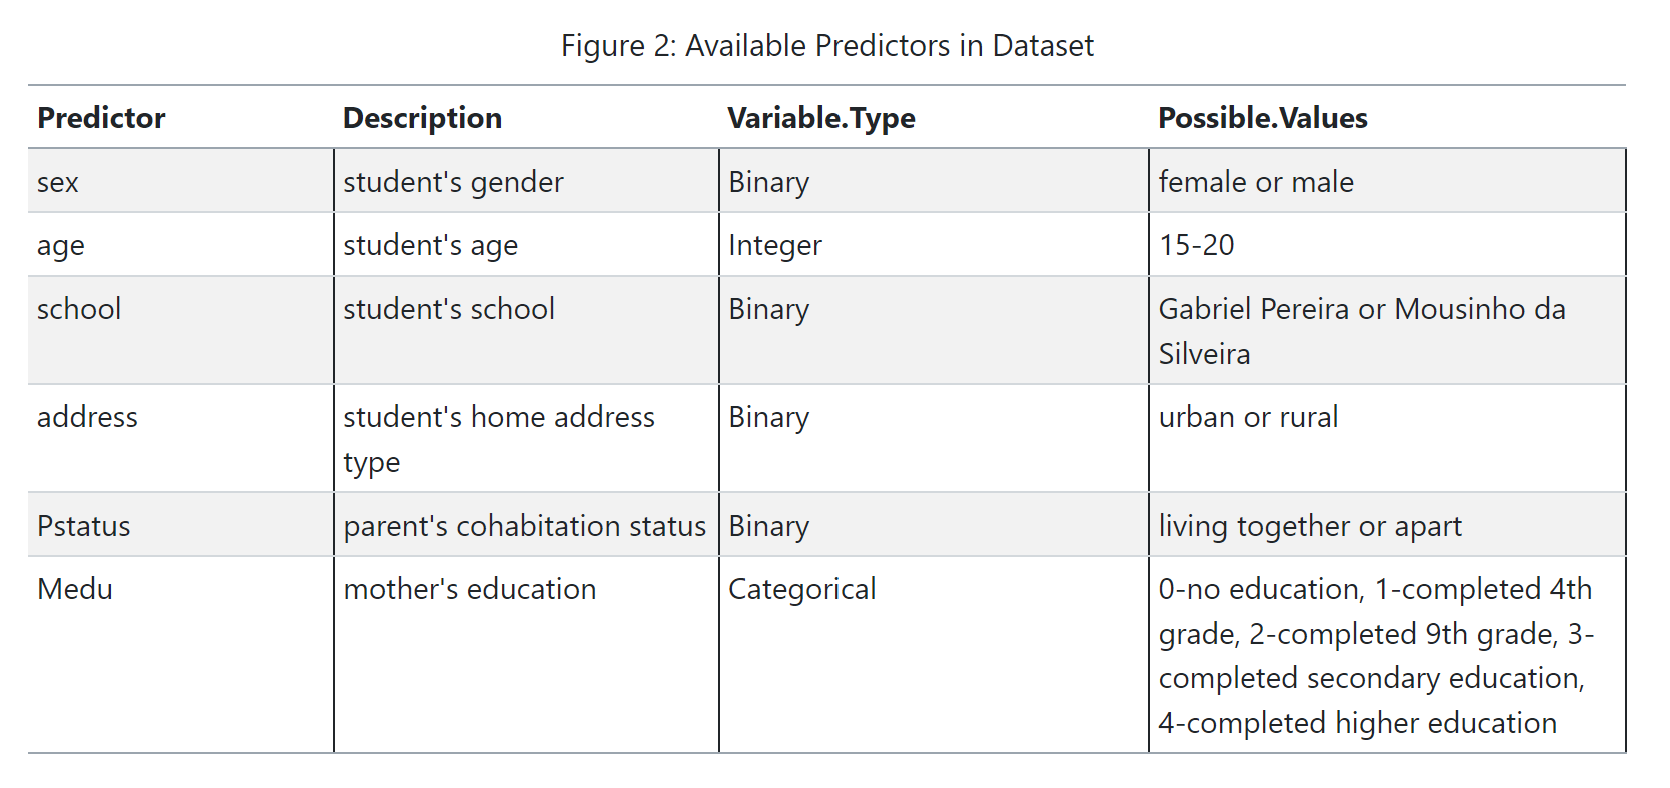
\includegraphics{predictor_examples.png}

First we examine scatterplots of G3 vs.~G1 and G2. We can observe a
clear linear correlation between the response and both predictors in
\textbf{Figure 3}. We can also observe that outliers exist where
students who recieved varying grades for G2 and G3 suddenly received 0
grades for G3, contrasting the linear trend.

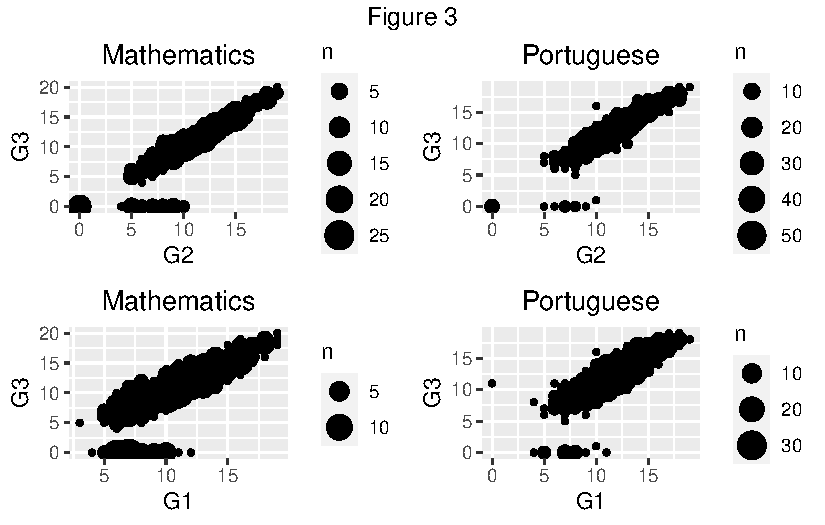
\includegraphics{Final_Paper_edit_files/figure-pdf/unnamed-chunk-2-1.pdf}

In \textbf{Figure 4}, we examine the relationship between G3 and the
predictors absences and failures. We can see a correlation between
absences and G3 but it is not linear. This suggests a transformation is
needed to appropriately fit absences into a linear model. We will use a
square root transformation as this is normal practice when dealing with
a count variable such as number of absences. We can observe that
failures only takes on values 0-3 so although it may seem similar to
absences in terms of being count data we will treat it as a categorical
variable and thus not apply a transformation.

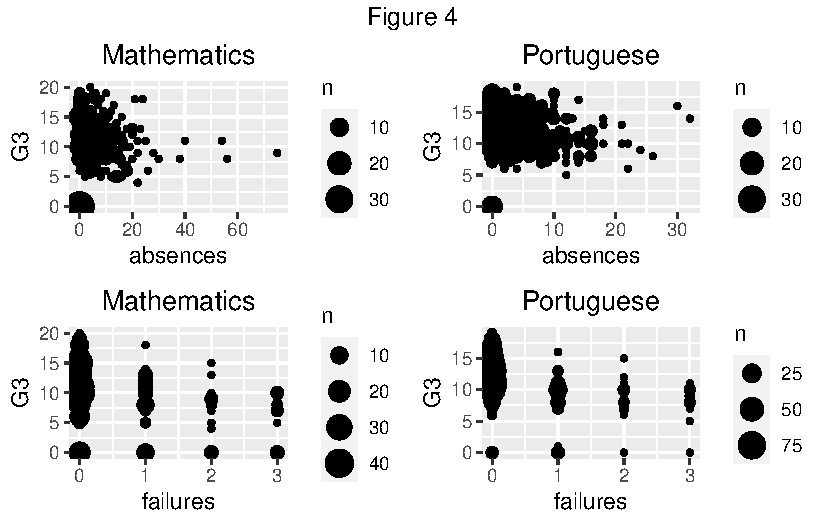
\includegraphics{Final_Paper_edit_files/figure-pdf/unnamed-chunk-3-1.pdf}

\subsection{Methods and Results}\label{methods-and-results}

Now we will construct our full model containing all predictors in our
dataset, appropriately classifying all categorical variables as factors
in R.

\begin{verbatim}
Figure 5: Summary for Mathematics Model 
\end{verbatim}

\begin{verbatim}
Significant Coefficients:
            Estimate Std. Error   t value     Pr(>|t|)
age       -0.2167846 0.10062393 -2.154403 3.194768e-02
failures1 -0.9389238 0.32994127 -2.845730 4.714093e-03
absences   0.4292284 0.06921107  6.201731 1.706608e-09
G1         0.2064483 0.06139562  3.362589 8.649267e-04
G2         0.9228330 0.05252456 17.569552 5.701784e-49

R-squared:  0.8726161 
Adjusted R-squared:  0.8446153 
F-statistic:  31.16396  on  71  and  323  DF, p-value:  8.483994e-109 

GVIF for provided predictors:
G1 :  5.016762 
G2 :  4.71554 
\end{verbatim}

\begin{verbatim}
Figure 6: Summary for Portuguese Model 
\end{verbatim}

\begin{verbatim}
Significant Coefficients:
               Estimate Std. Error   t value     Pr(>|t|)
reasonother -0.36219563 0.17468951 -2.073368 3.858122e-02
traveltime4  0.78846906 0.34980198  2.254044 2.456777e-02
failures1   -0.53967035 0.18770903 -2.875037 4.188834e-03
Dalc4       -0.84274543 0.35158917 -2.396961 1.684879e-02
absences     0.09847597 0.04307662  2.286065 2.261203e-02
G1           0.13739308 0.03868280  3.551788 4.138774e-04
G2           0.85282116 0.03632078 23.480255 4.447773e-86

R-squared:  0.867014 
Adjusted R-squared:  0.8506501 
F-statistic:  52.98315  on  71  and  577  DF, p-value:  4.063962e-209 

GVIF for provided predictors:
G1 :  4.688056 
G2 :  4.655541 
\end{verbatim}

In \textbf{Figure 5} and \textbf{Figure 6} we observe that our models
explain more than 80\% of the variance for their respective classes. G1
and G2 are very significant in both with low p-values. Absences is
significant and having 1 previous class failure is also significant. The
variables reason, traveltime, age, and Dalc (Weekday alcohol
consumption) disagree between the classes on their significance in
predicting G3. This could be a true population difference between
academic subjects, but the relatively high p-values of these variables
leads us to hypothesize these variables are not actually significant.

We also can see the generalized variance inflation factors (GVIFs) for
G1 and G2 are high, showing a likely issue with multicollinearity. This
is reasonable since our hypothesis is that prior grades predict future
grades, so it would naturally follow that G1 and G2 are highly
correlated.

Next we will examine our model diagnostics for the full model.

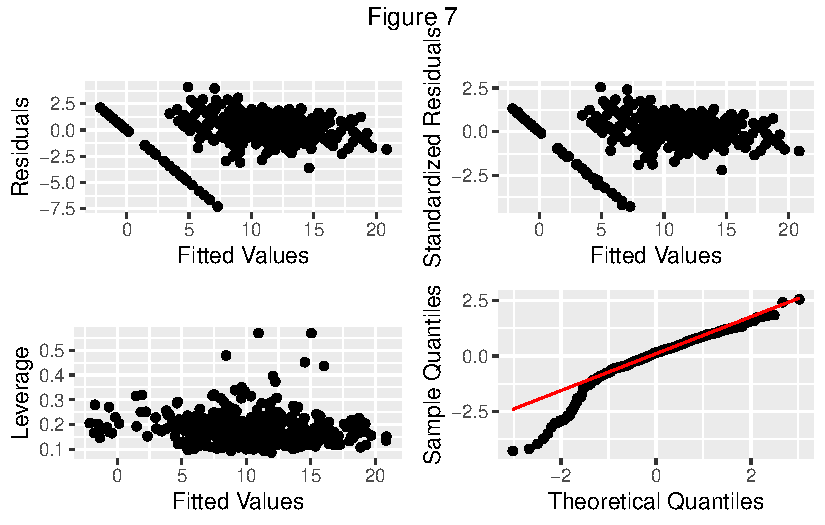
\includegraphics{Final_Paper_edit_files/figure-pdf/unnamed-chunk-7-1.pdf}

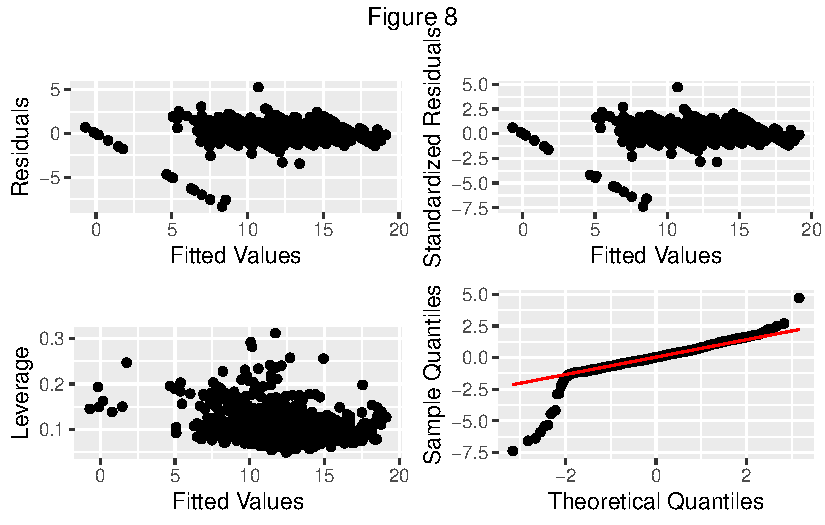
\includegraphics{Final_Paper_edit_files/figure-pdf/unnamed-chunk-7-2.pdf}

\textbf{Figure 7} and \textbf{Figure 8} show a clear division in the
distribution of points in the plots of standardized residuals vs.~fitted
values. One set demonstrates relatively constant variance, and the other
shows a clear linear pattern in its variance. Additionally we can see
that the QQ plot shows drop off from rest of the points on the lower end
of Theoretical Quantiles, meaning the sample quantiles are much lower
than what we would expect from normally distributed data.

To further examine our assumption of normality we will apply the
Shapiro-Wilk test to both classes.

\begin{Shaded}
\begin{Highlighting}[]
\FunctionTok{cat}\NormalTok{(}\StringTok{"Figure 9 }\SpecialCharTok{\textbackslash{}n}\StringTok{"}\NormalTok{)}
\end{Highlighting}
\end{Shaded}

\begin{verbatim}
Figure 9 
\end{verbatim}

\begin{Shaded}
\begin{Highlighting}[]
\FunctionTok{shapiro.test}\NormalTok{(}\FunctionTok{rstandard}\NormalTok{(lm\_full\_math))}
\end{Highlighting}
\end{Shaded}

\begin{verbatim}

    Shapiro-Wilk normality test

data:  rstandard(lm_full_math)
W = 0.91826, p-value = 8.046e-14
\end{verbatim}

\begin{Shaded}
\begin{Highlighting}[]
\FunctionTok{shapiro.test}\NormalTok{(}\FunctionTok{rstandard}\NormalTok{(lm\_full\_port))}
\end{Highlighting}
\end{Shaded}

\begin{verbatim}

    Shapiro-Wilk normality test

data:  rstandard(lm_full_port)
W = 0.81994, p-value < 2.2e-16
\end{verbatim}

\textbf{Figure 9} gives p-values for both classes that allow us to
reject the null hypothesis that are residuals are normally distributed.
Although the W values may allow us to claim that the full mathematics
model may satisfy our assumptions enough to draw conclusions, we see a
lower W value for the full portuguese model which was constructed from
more observations than the mathematics model.

Our diagnostics of the full multiple linear regression models showed
multiple issues. These issues as discussed above, alongside non-normal
results from Shapiro-Wilk tests and relatively high GVIF values provides
evidence that our assumptions for MLR Regression in the full model are
not satisfied. This leads us to attempt to reduce and adjust our full
model into a model that will improve our diagnostics.

Due to the large number of potentially important variables in our data
sets, we elected to use an algorithm-based approach to create our
reduced models. However, the diagnostics for both reduced models
resulted QQ and residual plots with similar issues to the full model.

Investigation into the points of the deviant standardized residual line
for both models revealed that the 22 of 24 (Portuguese: 8/10,
Mathematics: 14/14) had drop offs of their G3 grade to 0, and all 24 had
no absences recorded. There is not information about what these 0s
entail in the data set, nor in the research article where the data set
was obtained. It is possible that these outliers were data entry errors,
a non-pass being entered as a 0 instead of the actual G3 grade. However,
this is only speculation and, per the article, students were ``dropped
due to missing data''.

Because of these facts, we decided to remove the points that exhibited
the drop off of the G3 grade from the data sets due to the large bias
caused by outliers and the lack of clarity on these points validity to
the study.

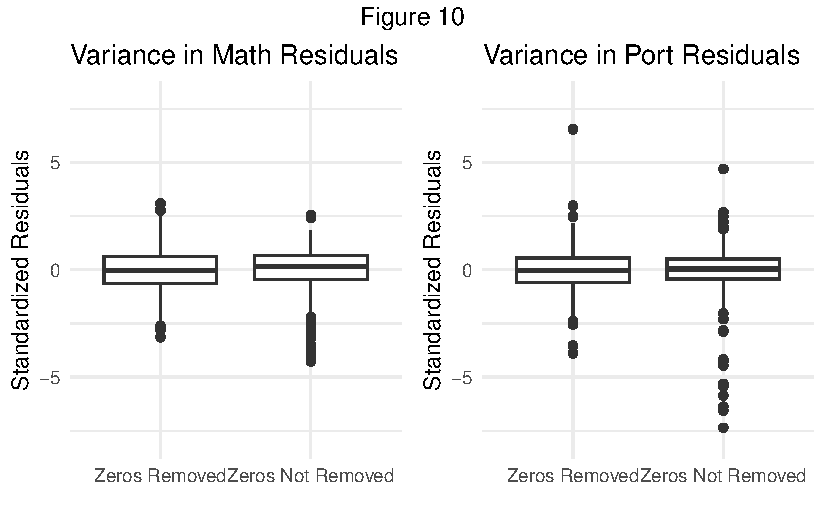
\includegraphics{Final_Paper_edit_files/figure-pdf/unnamed-chunk-10-1.pdf}

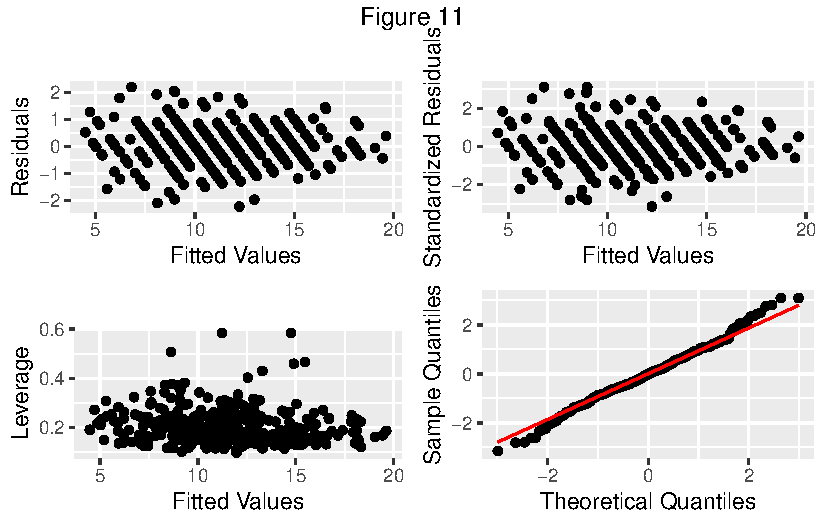
\includegraphics{Final_Paper_edit_files/figure-pdf/unnamed-chunk-11-1.pdf}

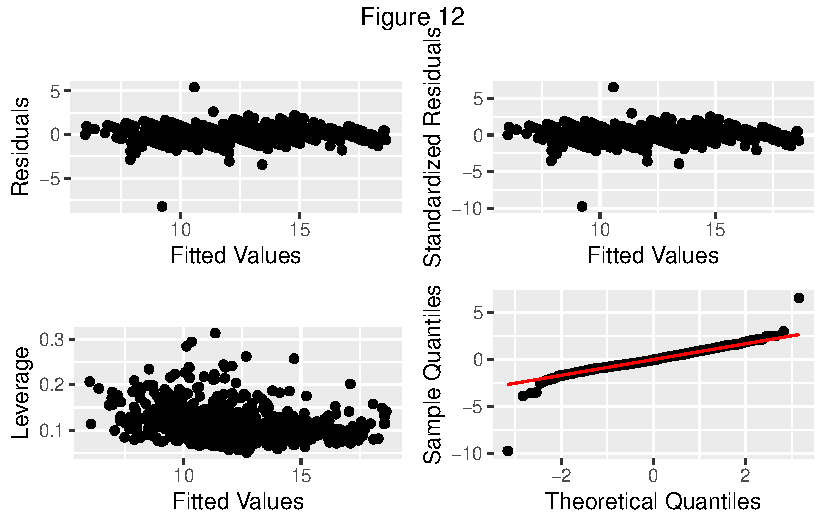
\includegraphics{Final_Paper_edit_files/figure-pdf/unnamed-chunk-11-2.pdf}

From the box plots in \textbf{Figure 10} we can see that there is a
clear improvement in how uniformly dispersed the standardized residuals
are once we remove the rows where G3 = 0. In \textbf{Figure 11} and
\textbf{Figure 12} we also see improvement in our diagnostic plots, and
apart from a few outlying points, most of the residuals seem randomly
distributed with constant variance. However there appears to be a
fundamental pattern in the residuals where they are divided into
discrete groups that are arranged diagonally. This is actually a
reasonable outcome since our response variable is a discrete integer.
Thus it follows that each increment in G3 will have its own group of
residual points distributed around it.

Nonetheless this is a fundamental problem with our approach because a
linear model assumes a continuous relationship between response and
predictors. One way of solving this is to change our response variable
into an average of the three grade variables (G1, G2, and G3).

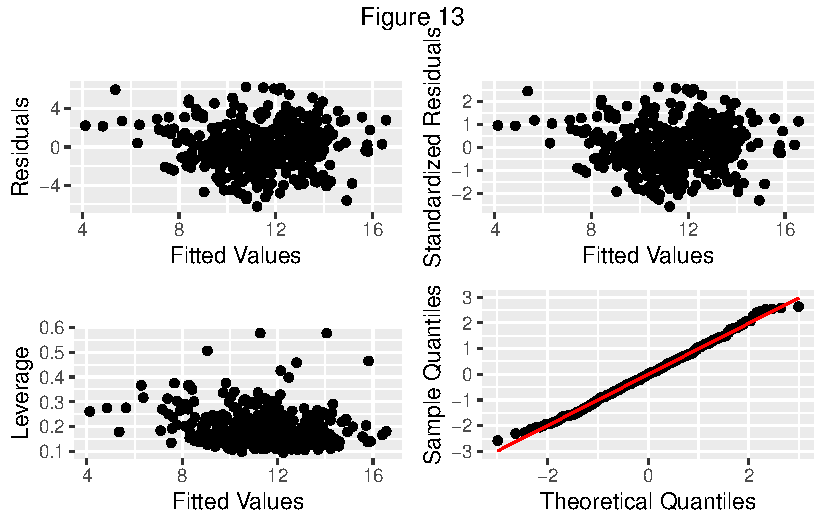
\includegraphics{Final_Paper_edit_files/figure-pdf/unnamed-chunk-12-1.pdf}

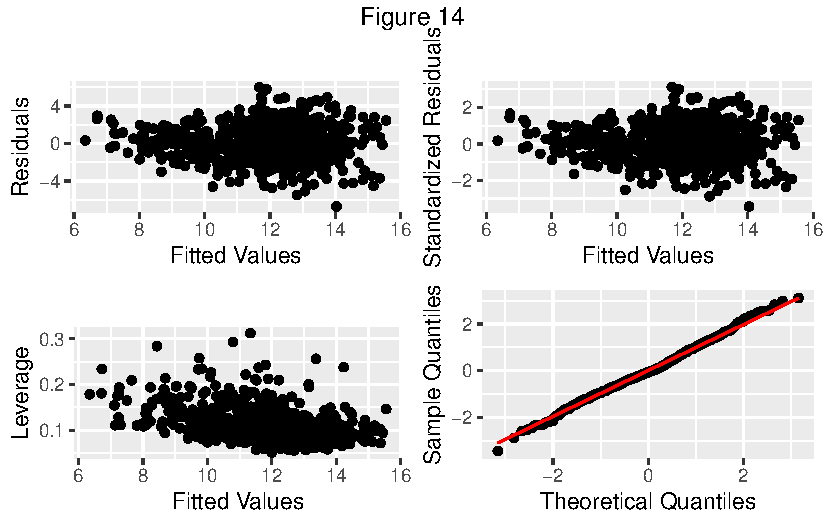
\includegraphics{Final_Paper_edit_files/figure-pdf/unnamed-chunk-12-2.pdf}

As we can see in \textbf{Figures 13 and 14}, the residuals are no longer
in a set of diagonal patterns, meaning that our linear regression
assumptions may be valid for these models. One the other hand, we have
sacrificed our most significant predictors (G1 and G2) and it is likely
these models will not explain as much of the variance in GPA as are
previous models did with G3.

\begin{verbatim}
Figure 15: Summary for Reduced Mathematics Model 
\end{verbatim}

\begin{verbatim}
Significant Coefficients:
               Estimate Std. Error   t value     Pr(>|t|)
(Intercept)  14.3787365  1.0802483 13.310585 1.336609e-32
sexM          0.6538912  0.3145877  2.078566 3.843670e-02
Mjobhealth    1.7742185  0.6286054  2.822468 5.057305e-03
Mjobservices  1.2366072  0.4856457  2.546316 1.134482e-02
studytime3    1.1121153  0.4943670  2.249574 2.514078e-02
studytime4    1.4192375  0.6444916  2.202104 2.835566e-02
failures1    -1.2763254  0.4976691 -2.564606 1.077532e-02
failures2    -2.4552254  0.8530506 -2.878171 4.263105e-03
failures3    -3.4877791  0.8570681 -4.069431 5.913990e-05
schoolsupyes -2.0909554  0.4291309 -4.872535 1.720352e-06
famsupyes    -0.7231220  0.3049584 -2.371215 1.830875e-02
health3      -1.6037258  0.5095535 -3.147316 1.799429e-03
health4      -1.0925124  0.5464915 -1.999139 4.642055e-02
health5      -1.3146756  0.4730484 -2.779156 5.765207e-03
absences     -0.3168997  0.1027885 -3.083027 2.223480e-03

R-squared:  0.347129 
Adjusted R-squared:  0.2892291 
F-statistic:  5.995331  on  29  and  327  DF, p-value:  2.314663e-17 
\end{verbatim}

\begin{verbatim}
Figure 16: Summary for Reduced Portuguese Model 
\end{verbatim}

\begin{verbatim}
Significant Coefficients:
                 Estimate Std. Error   t value     Pr(>|t|)
(Intercept)     6.4453534 1.67247052  3.853792 1.288831e-04
schoolMS       -0.9448490 0.19681446 -4.800709 2.000097e-06
sexM           -0.6019816 0.17984094 -3.347300 8.672519e-04
age             0.2480849 0.07849408  3.160555 1.654291e-03
Fjobteacher     1.2793288 0.49557161  2.581522 1.007346e-02
guardianmother -0.4110824 0.19829248 -2.073111 3.858961e-02
traveltime4    -1.2853433 0.53593022 -2.398341 1.677493e-02
studytime3      0.6854127 0.27563764  2.486644 1.316715e-02
studytime4      0.9970648 0.38685651  2.577351 1.019446e-02
failures1      -1.8830489 0.29520891 -6.378699 3.577825e-10
failures2      -2.7206480 0.56727597 -4.795987 2.046013e-06
failures3      -2.4942695 0.59429103 -4.197051 3.115044e-05
schoolsupyes   -1.1818250 0.27687669 -4.268416 2.288935e-05
higheryes       1.6447484 0.29916989  5.497707 5.704702e-08
goout2          0.9004455 0.35731720  2.520017 1.199418e-02
health5        -0.5180421 0.25963638 -1.995260 4.646778e-02
absences       -0.3198224 0.06776225 -4.719773 2.943331e-06

R-squared:  0.4154338 
Adjusted R-squared:  0.38122 
F-statistic:  12.14231  on  35  and  598  DF, p-value:  1.396738e-49 
\end{verbatim}



\end{document}
